\documentclass[a4paper,12pt,fleqn,oneside]{article} 
%\documentclass[a4paper,12pt,fleqn,oneside]{article} 	% Openright aabner kapitler paa hoejresider (openany begge)

%===== Projekt konstanter =====
\newcommand{\kursusTitel}{Semesterprojekt 4}
\newcommand{\linje}{IKT}
\newcommand{\semester}{4}
\newcommand{\system}{CarnGo}
\newcommand{\rapportType}{Projekt}
\newcommand{\gruppeNr}{5}
\newcommand{\vejleder}{Jesper Michael Kristensen, Lektor}
\newcommand{\afleveringsdato}{29. maj 2019}

%%%% PAKKER %%%%
% ¤¤ Oversaettelse og tegnsaetning ¤¤ %
\usepackage[utf8]{inputenc}					% Input-indkodning af tegnsaet (UTF8)
\usepackage[english, danish]{babel}			% Dokumentets sprog
\usepackage[T1]{fontenc}					% Output-indkodning af tegnsaet (T1)
\usepackage{ragged2e,anyfontsize}			% Justering af elementer

% ¤¤ Figurer og tabeller (floats) ¤¤ %
\usepackage{wrapfig}                        % text wrapping
\usepackage{graphicx} 						% Haandtering af eksterne billeder (JPG, PNG, PDF)
\usepackage{caption}
\usepackage{subcaption}
\usepackage{multirow}
% Fletning af raekker og kolonner (\multicolumn og \multirow)
\usepackage{makecell}                       % Line breaks i tabelceller med \makecell{bla bla \\ bla bla}
\usepackage{colortbl} 						% Farver i tabeller (fx \columncolor, \rowcolor og \cellcolor)
\usepackage[dvipsnames,table,longtable,x11names]{xcolor}

%Tabel automatisk ny linje
\usepackage{array}
\newcolumntype{L}[1]{>{\raggedright\let\newline\\\arraybackslash\hspace{0pt}}m{#1}}
\newcolumntype{C}[1]{>{\centering\let\newline\\\arraybackslash\hspace{0pt}}m{#1}}
\newcolumntype{R}[1]{>{\raggedleft\let\newline\\\arraybackslash\hspace{0pt}}m{#1}}

% Definer farver med \definecolor. Se mere: http://en.wikibooks.org/wiki/LaTeX/Colors
\usepackage{flafter}						% Soerger for at floats ikke optraeder i teksten foer deres reference
\let\newfloat\relax 						% Justering mellem float-pakken og memoir
\usepackage{float}							% Muliggoer eksakt placering af floats, f.eks.
\usepackage{afterpage}
%\usepackage{scrextend}                      % labeling lister
\usepackage{chngcntr} % kontroller nummerering af floats
\counterwithin{figure}{section} % sæt nummerering efter sektion
\counterwithin{table}{section} % sæt nummerering efter sektion

% ¤¤ Matematik mm. ¤¤
\usepackage{amsmath,amssymb,stmaryrd} 		% Avancerede matematik-udvidelser
\usepackage{mathtools}						% Andre matematik- og tegnudvidelser
\usepackage{textcomp}                 		% Symbol-udvidelser (f.eks. promille-tegn med \textperthousand )
\usepackage{siunitx}						% Flot og konsistent praesentation af tal og enheder med \si{enhed} og \SI{tal}{enhed}
\sisetup{output-decimal-marker = {,}}		% Opsaetning af \SI (DE for komma som decimalseparator)

% ¤¤ Misc. ¤¤ %
\usepackage{listings}						% Placer kildekode i dokumentet med \begin{lstlisting}...\end{lstlisting}

%Custom C Code Style
\lstdefinestyle{customc}{
    breaklines=true,
    language=[Sharp]C,
    basicstyle=\small\sffamily,
    numbers=left,
    numberstyle=\tiny\color{gray},
    frame=tb,
    columns=fullflexible,
    showstringspaces=false,
    keywordstyle=\bfseries\color{orange!40!black},
    commentstyle=\itshape\color{green!40!black},
    identifierstyle=\color{black},
    stringstyle=\color{purple},
    morekeywords={ abstract, event, new, struct,
    as, explicit, null, switch,
    base, extern, object, this,
    bool, false, operator, throw,
    get, set,
    break, finally, out, true,
    byte, fixed, override, try,
    case, float, params, typeof,
    catch, for, private, uint,
    char, foreach, protected, ulong,
    checked, goto, public, unchecked,
    class, if, readonly, unsafe,
    const, implicit, ref, ushort,
    continue, in, return, using,
    decimal, int, sbyte, virtual,
    default, interface, sealed, volatile,
    delegate, internal, short, void,
    do, is, sizeof, while,
    double, lock, stackalloc,
    else, long, static,
    enum, namespace, string},
}


\usepackage{blindtext}
\usepackage[legalpaper, portrait, margin=1in]{geometry}
\usepackage{lipsum}							% Dummy text \lipsum[..]
\usepackage[shortlabels]{enumitem}			% Muliggoer enkelt konfiguration af lister
\usepackage{pdfpages}						% Goer det muligt at inkludere pdf-dokumenter med kommandoen \includepdf[pages={x-y}]{fil.pdf}
\usepackage[bottom]{footmisc}               % Saetter footnotes i bunden af siden
\pdfoptionpdfminorversion=6					% Muliggoer inkludering af pdf dokumenter, af version 1.6 og hoejere
\pretolerance=2500 							% Justering af afstand mellem ord (hoejt tal, mindre orddeling og mere luft mellem ord)


%%%% BRUGERDEFINEREDE INDSTILLINGER %%%%

\linespread{1,1}							% Linie afstand

% ¤¤ Visuelle referencer ¤¤ %
\usepackage[colorlinks,pdfencoding=auto]{hyperref}			% Danner klikbare referencer (hyperlinks) i dokumentet.
\hypersetup{colorlinks = true,				% Opsaetning af farvede hyperlinks (interne links, citeringer og URL)
    linkcolor = black,
    citecolor = black,
    urlcolor = black
}

%%%% TODO-NOTER %%%%
\usepackage[danish, colorinlistoftodos]{todonotes}
%\usepackage[colorinlistoftodos]{todonotes}

%%%% TABEL BAGGRUNDSFARVER %%%%
\definecolor{aublueclassic}{RGB}{0,61,115}
\definecolor{aubluedark}{RGB}{0,37,70}
\definecolor{aucyan}{RGB}{225,248,253}
%\definecolor{aucyan}{RGB}{55,160,203}
\definecolor{aucyandark}{RGB}{0,62,92}
\definecolor{lightGray}{RGB}{153,153,153}
\definecolor{darkGray}{RGB}{119,119,119}
\definecolor{khaki}{RGB}{240,230,140}
\definecolor{lavender}{RGB}{230,230,250}

%indentering af section
\usepackage{changepage}

%Code highlighting
\usepackage{minted}

%%%% Tabs %%%%
\usepackage{tabto}
\NumTabs{10}

%%%% REFERENCE TIL SECTION-NAME %%%%
\usepackage{nameref}
\newcommand*{\fullref}[1]{\textbf{\ref{#1} \nameref{#1}}} % One single link

%sidehoved
\usepackage{fancyhdr}
\usepackage{lastpage}

%referer til afsnit i andre dokumenter
\usepackage{xr}

%MANGLER AT FIKSE DETTE 
\externaldocument[arch:]{aux_files/Arkitektur}
\externaldocument[accepttestspec:]{aux_files/Accepttestspecifikation}
\externaldocument[hwdesign:]{aux_files/HardwareDesign}
\externaldocument[analyse:]{aux_files/Analyse}
\externaldocument[integration:]{aux_files/Integrationstest}
\externaldocument[kravspec:]{aux_files/Kravspecifikation}
\externaldocument[modultest:]{aux_files/Modultest}
\externaldocument[proces:]{aux_files/Procesdokument}
\externaldocument[swdesign:]{aux_files/Softwaredesign}

%%%% biblatex %%%%
\usepackage[backend=bibtex,style=ieee]{biblatex}
\bibliography{Litteratur} 

%%%% KRAV numerering %%%%

\newcounter{req} \setcounter{req}{0}
\newcounter{subreq}[req] \setcounter{subreq}{0}
 
\renewcommand{\thereq}{\arabic{req}}
\renewcommand{\thesubreq}{\arabic{req}.\arabic{subreq}}
 
\newenvironment{req}[1]%
{
\refstepcounter{req}{K\thereq}}{}
\newenvironment{subreq}[1]%
{
\refstepcounter{subreq}{\noindent K\thesubreq}}{}


%%%% paragraph %%%%
%\usepackage{titlesec}
%\setcounter{secnumdepth}{4}

%\titleformat{\paragraph}
%{\normalfont\normalsize\bfseries}{\theparagraph}{1em}{}
%\titlespacing*{\paragraph}
%{0pt}{3.25ex plus 1ex minus .2ex}{1.5ex plus .2ex}

% ========== PAKKER DER SKAL LOADES TIL SIDST ==================
%\usepackage{xcolor}
%\usepackage{listings}
\usepackage{csquotes}           %så holder bilatex kæft
\usepackage{subfiles}


%%EDS SHIT
\PassOptionsToPackage{unicode=true}{hyperref} % options for packages loaded elsewhere
\PassOptionsToPackage{hyphens}{url}
%
\usepackage{lmodern}
\usepackage{amssymb,amsmath}
\usepackage{ifxetex,ifluatex}
\ifnum 0\ifxetex 1\fi\ifluatex 1\fi=0 % if pdftex
  \usepackage[T1]{fontenc}
  \usepackage[utf8]{inputenc}
  \usepackage{textcomp} % provides euro and other symbols
\else % if luatex or xelatex
  \usepackage{unicode-math}
  \defaultfontfeatures{Ligatures=TeX,Scale=MatchLowercase}
\fi
% use upquote if available, for straight quotes in verbatim environments
\IfFileExists{upquote.sty}{\usepackage{upquote}}{}
% use microtype if available
\IfFileExists{microtype.sty}{%
\usepackage[]{microtype}
\UseMicrotypeSet[protrusion]{basicmath} % disable protrusion for tt fonts
}{}
\IfFileExists{parskip.sty}{%
\usepackage{parskip}
}{% else
\setlength{\parindent}{0pt}
\setlength{\parskip}{6pt plus 2pt minus 1pt}
}
\usepackage{hyperref}
\hypersetup{
            pdfborder={0 0 0},
            breaklinks=true}
\urlstyle{same}  % don't use monospace font for urls
\usepackage{longtable,booktabs}
% Fix footnotes in tables (requires footnote package)
\IfFileExists{footnote.sty}{\usepackage{footnote}\makesavenoteenv{longtable}}{}
\setlength{\emergencystretch}{3em}  % prevent overfull lines
\providecommand{\tightlist}{%
  \setlength{\itemsep}{0pt}\setlength{\parskip}{0pt}}
% Redefines (sub)paragraphs to behave more like sections
\ifx\paragraph\undefined\else
\let\oldparagraph\paragraph
\renewcommand{\paragraph}[1]{\oldparagraph{#1}\mbox{}}
\fi
\ifx\subparagraph\undefined\else
\let\oldsubparagraph\subparagraph
\renewcommand{\subparagraph}[1]{\oldsubparagraph{#1}\mbox{}}
\fi

% set default figure placement to htbp
\makeatletter
\def\fps@figure{htbp}
\makeatother

\def\titlename{Proces}

\begin{document}

%===============FORSIDE======================
\pagestyle{fancy}
\fancyhf{}
\lhead{\kursusTitel\\Gruppe \gruppeNr}
\rhead{\titlename\\ \nouppercase{\leftmark}}
\lfoot{\afleveringsdato\\}
\rfoot{Side \thepage\space af \pageref{LastPage}}

\begin{titlepage}

\newcommand{\HRule}{\rule{\linewidth}{0.5mm}} % Defines a new command for the horizontal lines, change thickness here

\center % Center everything on the page
 
%----------------------------------------------------------------------------------------
%	HEADING SECTIONS
%----------------------------------------------------------------------------------------

\textsc{\LARGE Aarhus Universitet }\\[0.3cm] % Name of your university/college
\textsc{\Large \kursusTitel }\\[0.3cm]
\textsc{\Large Gruppe \gruppeNr }\\[0.5cm] % Major heading such as course name
 % Minor heading such as course title

%----------------------------------------------------------------------------------------
%	TITLE SECTION
%----------------------------------------------------------------------------------------

\HRule \\[0.4cm]
{ \huge \bfseries \titlename}\\[0.03cm]{\system} % Title of your document
\HRule \\[1.5cm]

 
%----------------------------------------------------------------------------------------
%	AUTHOR SECTION
%----------------------------------------------------------------------------------------

\begin{minipage}{0.4\textwidth}
\begin{flushleft} \small
\emph{Gruppemedlemmer:} 
\\Edward Hestnes Brunton\\ (201705579)
\\Marcus Gasberg\\ (201709164) 
\\Martin Gildberg Jespersen\\ (201706221) 
\\Mathias Magnild Hansen\\ (201404884)
\\Tristan Moeller\\ (201706862)
\\Erik Mowinckel\\ (20107667)
\\Hamza Ben Abdallah\\ (????????)
\\Alparslan Esen\\ (201405877)
\end{flushleft}
\end{minipage}
~
\begin{minipage}{0.4\textwidth}
\begin{flushright} \small
%\emph{Antal tegn:}\\
%77466 (med mellemrum).
%(Microsoft Word konvertering fra PDF)
%\newline
%\newline

\emph{Vejleder:} \\
\vejleder \\ % Supervisor's Name
\end{flushright}
\end{minipage}\\[1cm]

% If you don't want a supervisor, uncomment the two lines below and remove the section above
%\Large \emph{Author:}\\
%John \textsc{Smith}\\[3cm] % Your name

%----------------------------------------------------------------------------------------
%	DATE SECTION
%----------------------------------------------------------------------------------------

{\large \afleveringsdato}\\[1cm] % Date, change the \today to a set date if you want to be precise

%----------------------------------------------------------------------------------------
%	LOGO SECTION
%----------------------------------------------------------------------------------------

\begin{figure}[H]
    \centering
    
\includegraphics[width=0.15\textwidth]{Setup/graphics/AU.png}
\end{figure}

\vfill
\end{titlepage}
\subfile{ProcesDokument/Versionshistorik/Versionshistorik.tex}\newpage
\tableofcontents \newpage 

\section{Forord}
Dette dokument er skrevet af PRJ4 gruppe 5, der er en projektgruppe udelukkende bestående af IKT-studerende fra Aarhus Universitet. Dokumentet er udarbejdet som en beskrivelse af den proces, gruppen har været igennem under hele semesteret og har til formål at være en opsummering og sammekædning af procesrelateret information for forløbet, til hvem end det må interessere. Det ligger implicit, at for at forstå dette dokument må projektintroduktionen og noget af kravspecifikationen være læst på forhånd. Derudover fungerer dette dokument som en uddybning af Procesafsnittet. \\\\
Der er desuden hentet inspiration fra et tidligere projekt, PRJ3 Gruppe 7, da samme udviklingsværktøjer tages i brug. I det forrige projekt blev Scrum også brugt som et værktøj til at styre udviklingsprocessen. 

\section{Indledning}
I dette dokument beskrives alle procesrelaterende beslutninger i løbet af projektets udfoldelse.
Der berettes om gruppens dannelse, og hvordan arbejdsprocessen mellem gruppemedlemmerne har udviklet sig gennem flere iterationer. Der beskrives, hvilke udviklingsværktøjer og udviklingsmetoder, som er brugt til udarbejdelse af projektet. Dette vedrører bl.a. projektets ledelse, arbejdsfordelingen mellem projektets medlemmer og planlægning af møder. Til slut redegøres der eventuelle konflikthåndteringer. 

\section{Gruppedannelse}
På 4. Semester var der frit valg ved gruppedannelse, hvor det eneste krav var, at der var 7-8 medlemmer i gruppen. Gruppen måtte bestå af både IKT- og E-studerende, dog skulle der søges tilladelse, hvis begge studieretninger indgik i gruppen. Der var 5 IKT-studerende fra et tidligere semesterprojekt, som valgte at danne en gruppe. De resterende 3 medlemmer kendte allerede hinanden fra et tidligere semester og søgte en semestergruppe. Slutresultatet blev en gruppe med udelukkende IKT-studerende. \\
I de forrige semesterprojekter har der været benyttelse af Insights profiler til at identificere de roller, man skal udfylde jobmæssigt, samt som et redskab til at give selvindsigt i, hvordan man opnår bedre kommunikation mellem medlemmer. Tabel \ref{table_group_types} viser hvilken personlighedstype, de forskellige medlemmer er, samt deres adfærdstræk og attitudefarve. 

\begin{table}[H]
\centering
\begin{tabular}{|L{0.2\textwidth}|L{0.2\textwidth}|L{0.4\textwidth}|}
\hline
\textbf{Navn} & \textbf{Farve} & \textbf{Type} \\ \hline
Hamza Ben Abdallah & Gul & Hjælpende Inspirator \\ \hline
Tristan & Gul & Inspirerende Motivator\\ \hline
Mathias & Grøn & Supporter \\ \hline
Edward & Blå & Reformerende Observator \\ \hline
Martin G.J. & Blå  & Observatør \\ \hline
Erik Mowinckel & ?? & ??  \\ \hline
Alparslan & ?? & ?? \\ \hline
Marcus & Gul & Inspirator \\ \hline
\end{tabular}
\caption{Sammensætning af Insights typer i gruppen}
\label{table_group_types}
\end{table}

\section{Udviklingsforløb}
\subsection{Introduktion}
Dette afsnit omhandler den generelle beskrivelse af udviklingforløbet på PRJ4. Aarhus Universitet har angivet følgende krav for dette semesters projektudfoldelse. Gruppen skal: 
\begin{enumerate}
    \item Anvende en iterativ udviklingsproces
    \item Kombinere viden fra flere af semestrets kurser og anvende denne i projektet
    \item Anvende projekt- og versionsstyringsværktøjer
    \item Det gælder desuden, at forløbet er gruppebaseret og der er meget frie rammer for den måde, hvorpå den enkelte gruppe vælger at håndtere såvel proces som produktudvikling
    \end{enumerate}
Det angives frie rammer for projektets udfoldelse, dog med den betingelse at der anvendes en iterativ udviklingsproces, og læringsmålene opfyldes. I de næste afsnit beskrives, hvilke udviklingsmetode og udviklingsværktøjer der anvendes, og hvordan det anvendes. For de enkelte krav for læringsmål refereres til projektoplaget fra Aarhus Universitet. 

\subsection{Scrum}
Til forskel for de tidligere semestre har der ikke været noget krav om udviklingsmetoder til proces med den undtagelse, at der skulle anvendes en iterativ udviklingsproces. Det blev hurtigt besluttet at anvende Scrum, da flere medlemmer af gruppen havde god erfaring med dets fleksible og adaptive tilgang til arbejdsprocessen i form af korte iterationer med effektiv feedback mekanisme, samt gruppen havde allerede en tilpasset version af Scrum, udarbejdet i et af de tidligere semesterprojekter. Desuden var Scrum et krav for 3. semesterprojektet, så alle medlemmer har erfaring med det. \\
I det følgende afsnit beskrives, hvordan gruppen har benyttet Scrum som udviklingsværktøj. Den metodik som anvendes tager udgangspunkt i den tilpasset version af Scrum anvendt fra et tidligere semesterprojekt. For en mere dybdegående version af dette, refereres til Bilag \cite{Scrum}.

\subsubsection{Sprints}
For hvert iteration af projektets udarbejdelse er der et antal opgaver, som anstilles af gruppen og skal uddelegeres til en eller flere gruppemedlemmer. Til udførelse af ens opgaver er der tildelt en tidsperiode, hvor hvert medlem i gruppen arbejder på at fuldføre opgaverne. Hvert iteration eller et såkaldt sprint varer typisk mellem 1-2 uger. Ideelt set skal alle opgaver være løst ved slutningen af sprintet, således de kan gennemlæses, analyseres og vurderes af andre gruppemedlemmer - den specifikke fremgangsmetode beskrives længere nede i dokumentet. \\
Sprintenes varighed er mellem 1-2 uger pga. den varierende arbejdsmængde og fokus. De korte 1 ugers sprints blev generelt brugt til refaktoerisering af tidligere arbejde eller opgaver, som har været vanskelige at vurdere - generelt opgaver, som var mere målrettede. \\
Det kræver et stort overblik at lave opgaver nok til et hold bestående af 8 mennesker, og det blev forkastet at have sprints længere end 2 uger. Ved længere forløb mistes evnen til at estimere omfanget af opgaver samt at vurdereringen af projektets status og de individuelle medlemmers arbejdsindsats - det er lettere at korrigere et 2 ugers sprint, end et på 3-4 uger (fx hvis medlemmer ikke færdiggør tasks). Kommunikation er en fundamental faktor i projektarbejde, men det er ikke altid det letteste at opretholde - ved at have de korte sprints sikres det, at efter 1-2 uge opnås en konklusion: succes eller fiasko. 

\subsubsection{Rollerne i Scrum}
I dette afsnit beskrives de klassiske roller i Scrum, og hvordan det bliver realiseret i projektgruppen. I modsætning til forhenværende projektarbejde har vi ikke skiftet rollen som Scrum Master - efter erfaring blev det sjældent en flydende overgang, det endte blot med ingen tog ansvar med hensyn til Scrum Masterens opgaver og ledelse. I dette projekt blev Tristan Møller valgt som Scrum Master.

\textbf{Scrum Master} \\
En Scrum Master er en projektleder, som fokuserer på at optimere ydeevnen og arbejdet mellem produktets ejer og teamet, for at sikre konsekvente og succesrige sprints - og dette gøres bl.a. ved at faciliter Scrum i projektgruppen. Hans/Hendes opgave er at fjerne interne og eksterne forhindringer, således arbejdesprocessen optimeres for gruppen. Desuden skal Scrum Masteren også stå for de mere administrative opgaver, såsom at lave dagsordner, være bindeleddet mellem projektgruppe og vejleder og overholde deadlines. 

\textbf{Product Owner} \\
En Product Owner er ansvarlig for at maksimere værdien af produktet som følge af udviklingsholdets arbejde. Dette er bl.a. at sørger for, at produktets krav er klare og tydelige - angivet i Product Backlog. Her angives, hvad der vides at være nødvendigt for produktet, samt arbejdsopgavernes prioritet. Traditionelt repræsenterer Product Owner eksterne parters ønsker for produktet, fx en kunde, men da der ikke er nogen eksterne parter i dette semesterprojekt, udliciteres denne rolle til projektgruppen og eventuel vejleder. Prioritering af arbejdsopgaver vurderes fælles af projektgruppen. Det er dog ofte Scrum Masteren, som rankererer prioriteterne, da han/hende har et overblik over deadlines og de læringsmål, som er angivet af Aarhus Universitet for 4. semesterprojektet. 

\textbf{Team Member} \\
Et Team Member har til ansvar at fuldføre opgaver tildelt, således der arbejdes frem mod et færdigt projekt. Alle medlemmer i projektgruppe er et Team Member, også Scrum Masteren - dette betyder også at Scrum Master også har arbejdsopgaver, der ligger udenfor Scrum Masterens rolle. 

\subsubsection{Scrum Relaterede møder} 
Af Scrum kan der hives 4 møder ud: Daily Standup Meeting, Sprintplanlægning, Sprint Retrospective og Sprint Review. Da alle gruppens medlemmer samtidigt fungerer som studerende på Aarhus Universitet, var det allerede fra en start tydeligt, at det ville være urealistisk at holde et møde om dagen. Efter lidt gennemgang af kalenderen blev det fundet, at de eneste tidspunkter, det var muligt for begge studieretninger at mødes, var mandag eftermiddag og onsdag eftermiddag. Det blev derfor besluttet, at der inden hvert møde var et kort Standup Meeting, der havde til formål at opdatere alle parter om, hvad de andre lavede og hvor langt de var - dette gav Scrum Masteren det nødvendige overblik til at evaluere, om sprintets opgaver ville blive lavet, eller om medlemmer forsømte arbejdsopgaver. \\
Med 2 dages deadline blev det også tydeligt, at efter hvert sprint måtte laves et samlet møde for Sprint-Retrospektiv,-Review og -Planlægning. 

\subsubsection{Redskaber} 
\textbf{Visual Studio}\\
Microsoft Visual Studio er et integreret udviklingsmiljø fra Microsoft. VS bruges som hoved IDE'et i projektet, både til udviklingen af den grafiske brugeroverflade (WPF) og databasen (EF Core). 

\textbf{GitHub}\\
GitHub er en webbaseret hosting service til versionskontrol ved hjælp af Git. Et af kravene for semesterprojektet er versionsstyring. GitHub bruges i projektet til at versionstyre projektets dokumentation og sourcekode. GitHub er desuden integreret i Visual Studio, samt har en brugervenlig grænseflade til forskel for andre versionstyringsværktøjer. 

\textbf{Zenhub}\\
Det var essentielt for projektgruppen at have et redskab til at strukturere opgaverne, så det gav et klar overblik over de opgaver, som var aktive i sprintet, samt hvilke opgaver der var tildelt gruppemedlemmer - generelt et værktøj, som kunne skrædersys til projektets Scrum metodik. Aarhus Universitet anbefalede Zenhub, da det er et fleksibelt værktøj, samt muligt at integrere med GitHub - flere af gruppens medlemmer havde også god erfaring med det. \\
Et Zenhub projekt blev oprettet, og projektgruppens Scrum værdier og metoder blev integreret i den visuelle repræsentation af opgaverne: deres prioriet, arbejdsansvarlig og stadie. Projektet udgør en del af det fælles GitHub repository for gruppen, det er således muligt at gemme tidligere sprints. 

\textbf{Jenkins}\\
Applikation CarnGo, som udarbejdes i projektet, skal kontinuerligt testes for fejl i forhold til enhed- og integrationstests. I stedet for at hvert medlem skal teste dette lokalt på en computer, udliciteres dette til en 'build' server, som kompilerer holdets kode fra et delt versionstyringregister (GitHub). Jenkins er en CI build server, som automatiserer enhed- og integrationstests. Jenkins er open source, men er ofte kendt for dets svære opsætning og administration af servere. Aarhus Universitet har allerede oprettet en CI server via Jenkins, som Projektgruppen har valgt at udnytte - herved undgår gruppen at bruge unødvendig tid på at opsætte en server. For en mere uddybende beskrivelse af brugen af Jenkins serveren henvises til bilag Softwaretest.
\begin{figure}[H]
    \centering
    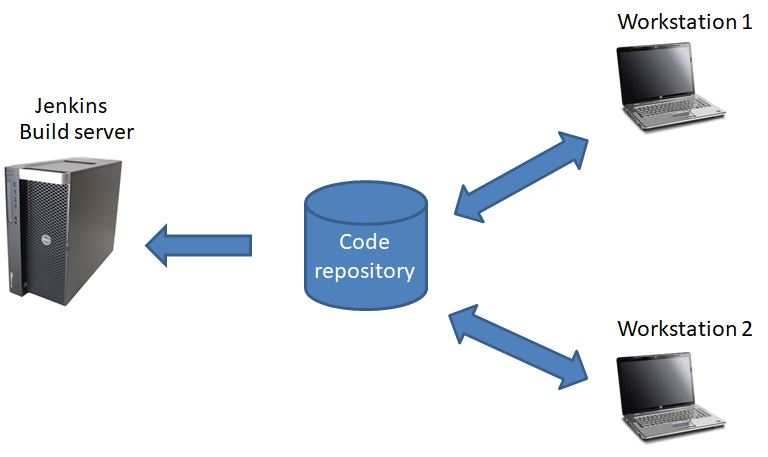
\includegraphics[width=\textwidth]{ProcesDokument/graphics/Jenkins.jpg}
    \caption{Continous Integration vba. af Jenkins Build Server}
    \label{fig:jenkins}
\end{figure}

\textbf{Overleaf}\\
Overleaf er en online LaTex editor, som gør det muligt at realtidssamarbejde og kompilering mellem flere brugere. Alle medlemmer var fortrolig med LaTex og enige om Overleaf var et exceptionelt værktøj og teksteditor.  

\textbf{Menderley}\\
Menderley bruges til at kompilere .bib filer, som bruges til at oprette referencer i LaTex. Menderley giver en drag and drop funktionalitet for bilag, som gør det let at tilføje bilag og andre referencer - desuden kan det integreres med Overleaf. 

\subsection{Erfaringer med Scrum}
Det er nu anden semester i træk, hvor der benyttes Scrum som proces- og udviklingsmetode. Der er dog stadig en masse nye teknologier, som skal undersøges og implementeres, men det at allerede være rutineret i Scrum har givet substantielt mere tid og effektiviseret arbejdsprocessen. Feedback mekanisme i form af udfaldet af hvert sprint iteration, er en essentiel faktor i at vurdere projektets nuværende position - her kan man løbende vurdere medlemmers indsats, samt hvilke opgaver, som skal prioriteres og uddelegere arbejdsressourcer - ofte faciliteret af Scrum Masteren eller Product Owner. 

Projektgruppen har også stiftet bekendskab til det Agile Manifest, som løbende er blevet inkorporeret i udøvelse af Scrum. Scrum anses allerede for at være et agilt udviklingsværktøj, men det er ikke giver ikke garanti for, at de agile værdier og principper overholdes.
Det Agile Manifest indebærer:  
\begin{itemize}
    \item Individer og interaktioner frem for processor og værktøjer
    \item Realiseret software frem for omfattende dokumentation 
    \item Kundesamarbejde over kontraktforhandling 
    \item Responderer til ændringer i stedet for at følge en statisk plan
\end{itemize}
Det er en central faktor at planlægge ens projekt og sprints, således man sikrer at nå alle krav for produktet/systemet. Vandfaldsmodellen er et godt eksempel på en statisk gennemgang af arbejdsiteration. Her antager man, at de forrige stadier er gennemførte, når man begynder på et nyt. Dette er sjældent tilfældet. Vi har benyttet sprints til at gå frem og tilbage mellem arbejdsstadier. For at kunne begynde på første udkast af design eller arkitektur, skal man have dokumenteret nok krav for produktet - og det er præcist det, som blev gjort. Når det besluttede af kravspecifikationen var forståelig og generel nok ("Just enough" som Martin Fowler ville sige), til at det var muligt at begynde på arkitekturen, vil næste sprints opgaver omhandle produktets arkitektur. Herefter vil man så kunne gå tilbage, hvis kravspecifikationen ikke var dybdegående nok til at arbejde videre på produktets arkitektur - disse iteration giver herved gruppen feedback og mulighed for at gå tilbage til tidligere stadier.
\begin{displayquote}
"Base your architecture on requirements, travel light and prove your architecture with concrete experiments."
"Provide the foundations and vision to move forward." \\
- Scott Ambler 
\end{displayquote}
Det skal dog ikke forveksles med at det er i orden at lave en utilstrækkelig opgave og antage, at det bliver færdiglavet i et senere sprint. Det hændte dog, at der opstod flere episoder, hvor dette skete og resulterede i, der måtte bruges et helt sprint på at fikse dette. Selvom der arbejdes iterativt og agilt, bør en arbejdsopgave stadig være tilstrækkelig færdig til at kunne arbejde videre på. Hvis der ikke er forudsætninger for at kunne udføre opgaven, skal der selvfølgelig ikke bruges ressourcer. Der er således en fin grænse mellem mangelfuld arbejdsindsats og en arbejdsopgave, som skal laves over flere iterationer.\\\\
Et sprint bruges således til at 'bevise' fx kravspecifikation. Dette resulterer i at enten forkastes det eller godkendes (dog åben for ændringer). Dette betyder, at man ikke er fastsat på krav, som ikke er testes eller anvendt og derved skaber større risiko for fejl. En anden faktor er, at det er lettere at skabe værdi for en kunde, da man gå frem og tilbage mellem design og implementation, kun en begrænset mængde skal være fastlåst. Generelt er den højeste prioritet at tilfredsstille kunden gennem tidlig og kontinuerlige leveringer af værdifuld software.

\subsubsection{Sprints}
I dette afsnit beskrives alle overordnede refleksioner og overvejelser for alle sprints under projektets udførelse. Det gennemgår nogle af de erfaringer, der er blevet gjort i løbet af anvendelse af Scrum. Her berettes omkring specifikke produkt- og procesbeslutninger. Til slut sammenfattes alle episoder i en konklusion - hvis man ikke ønsker at læse en dybdegående beskrivelse af hvert sprint, henvises læseren til konklusionen. 

\textbf{Sprint 1}\\
Dette var det indledende sprint for projektet. Det betød, der var en del formelle konventioner som skulle udføres:
\begin{enumerate}
    \item Vi skulle lære hinanden at kende
    \item Vi skulle høre om hinandens erfaringer med udviklingsværktøjer (Scrum) 
    \item Vi skulle etablere individuelle ønsker for projektets akademiske krav. 
\end{enumerate}
Vi havde alle erfaring med 3. semesters kaotiske start, hvor man skulle bruge overraskende meget energi på at integrere Scrum ind i ens arbejdsproces, samt finde værktøjer, som supplerede denne arbejdsform. Den første dag blev brugt på at definere fælles krav for hvilke overordnede værktøj, som skulle bruges. \\
Sprintet havde anticiperet resultat: gruppen er en blanding af medlemmer, som har arbejdet sammen før, samt helt nye medlemmer. Kommunikation var derfor et problem, hvor de nye medlemmer havde svært ved at følge med de andre medlemmer, som talte sammen på daglig basis - det var således essentielt at de 'gamle' medlemmer var bedre til at indrage de nye medlemmer i gruppen og kommunikerer bedre. 

\textbf{Sprint 2} \\
I dette sprint begynder Scrums iterative tilgang at træde i kraft. Der er uadarbejdet en kravspecifikation, som er beskrivende nok, og det betyder, vi begynder med arkitekturen. Det er bred enighed om, at kravspecifikation ikke er færdig, men det er nødvendigt at realisere arkitekturen for at undersøge, om kravene faktisk kan realiseres eller giver mening.\\\\
Der bliver etableret første udgave af et review/feedback system, hvor den sidste mandag i sprintet reserveres til at få en opgaver reviewet. Det er således medlemmets eget ansvar at få opgaver reviewet. 

\textbf{Sprint 3} \\
Der bliver startet et nyt sprint efter et ekstern review. Gruppen har fået at vide, at projektet skal afgrænses, da der er for høje ambitioner - desuden er der også givet feedback på kravspecifikationen. Dette sprint itereres da fra et arkitekturstadie til et sprint omhandlende krav og afgræsning. Sprint planlægningen er blevet bedre i form af folk udnyttet de værktøjer, som er opsat (Zenhub, Overleaf og GitHub). Det eksterne review er en kæmpe hjælp, projektet bliver substantielt afgrænset, og kravspecifikationen reflekterer dette inden sprintets slutning.  

\textbf{Sprint 4}\\
Det er Scrum Masterens ansvar at sikre, at alle leverer og laver deres arbejdsopgaver. Gruppemedlemmer dokumenterer ikke deres arbejde i Overleaf, det er derfor ikke muligt at se, hvad der bliver lavet. Der er enighed om i gruppen, at det ikke er Scrum Masterens ansvar at skrive til hvert person, hvis det viser sig, at opgaverne ikke bliver lavet. Det besluttes derfor, at det er obligatorisk at anvende de 2 timer, som er afsat til projektarbejde hver mandag og onsdag. Herved sikres, at alle arbejder minimum 4 timer i ugen, og der bruges tid på intern sparring. 

\textbf{Sprint 5}\\
Studiets arbejdsbyrde er begyndt at stige, og det afspejles i projektarbejdet, og der opleves en del sygdom og fravær. Det er tydeligt, at der er mangel på disciplin i forhold til projektet, og gruppen forsøger at opretteholde arbejdsindsatsen. Gruppemedlemmer bliver enige om, at der skal fokuseres på at anvende møderne til at lave opgaver, samt at alle ens opgaver skal være klar til review den sidste mandag i sprintet. Enkelte medlemmer benytter stadigvæk ikke Overleaf eller Zenhub til at angive status på deres tasks. Projektets medlemmer efterspørger Scrum Masteren til at skrive til personerne, som ikke benytter værktøjer - projektet er nået til det stadie, at det påvirker de andre medlemmers arbejde, og det er ikke acceptabelt at lave alt arbejdet dagen inden eller ikke at levere noget. 

\textbf{Sprint 6}\\
Møderne bliver udnyttet til at arbejde, dog med enkelte afvigelser. Enkelte medlemmer møder ikke op eller siger ved slutningen, at de ikke kunne lave deres opgaver, fordi de ikke kunne finde ud af det, men de har ikke efterspurgt hjælp. Der opfordres i dette sprint at fokusere på dokumentation, da der er en del mangler, som kommer til at udgøre en stor risiko for projektets færdiggørelse - der er mangel på en rød tråd gennem kravspecifikationen og arkitekturen. Enkelte medlemmer glemmer at se deres opgaver som en helhed, blot en opgave som skal løses og eventuelt færdiggøres i fremtiden. Dette kan resultere i et seriøst problem, men gruppens medlemmer gøres opmærksom på dette. 

\textbf{Sprint 7}\\
Dette sprint finder sted under påskeferien, så det aftales fra start, at alle skal være gode til at kommunikere og løbende dokumentere i Overleaf. Desværre lykkedes dette ikke, og enkelte medlemmer har været på ferie og ikke lavet deres opgaver. Der udvises stor forståelses, hvis man ønsker at holde ferie, men så skal man ikke påtage sig opgaver, man ikke kan klare. Der er således enkelte opgaver, som ikke bliver løst i dette sprint, som skal restribueres til andre medlemmer. Dette er på ingen måder ideelt, da tidligere vurderinger af projektets status må forkastes. Det ender dog med, at de fleste medlemmer bruger en del tid i slutningen af sprintet på at lave alle deres opgaver - det var dog ikke det gruppen håbet på, da mandagen helst skal bruges til review af arbejdet. 

\textbf{Sprint 8}\\
Der er nu kun 1 måned tilbage, før det første udkast af rapport skal værek klar. Retrospektiv for det forrige sprints mål har gjort det klar, at nogle medlemmer ikke laver deres tasks ordenlig, samt ikke sætter det ind i det store perspektiv. I starten af sprintet bliver gruppen enige om, at der skal sættes nogen rammer for projektet, som forhåbentligt skal gøre det klar for alle medlemmer, at der vil være konsekvenser, hvis man ikke udfører arbejdsopgaver:
\begin{enumerate}
    \item Hvert tasks skal tildeles en review partner. Review partneren står også til ansvar for udførelsens af opgaven og dets kvalitet. 
    \item Det er obligatorisk at bruge møderne til at arbejde, medmindre man har en rigtig god undskyldning (I så fald skal det også være leveret den mængde arbejde, svarende til 2 timer ifh. til mødet). 
    \item Hvis ikke dette opfyldes, skal medlemmet have en samtale med vejleder inden andre aktioner tiltages. 
\end{enumerate}
Udover dette så prioriteres dokumentation og integration af databasen. Det forrige sprint gav mulighed for at lave tests og tilføje features, men det er vurderet til at være for sent at gøre nu. 

\textbf{Sprint 9}\\
IKKE LAVET ENDNU 

\textbf{Konklusion på Scrum anvendelse i gruppen }\\
Gruppen har ikke formået at anvende den ideelle version af Scrum, men lavet et skræddersyet version, som passer gruppens arbejdsprocessor og tidsresourcer. Figur \ref{fig:scrum_usage} viser en illustration af hvordan gruppen har anvendt Scrum i semesterprojektet. 
\begin{figure}[H]
    \centering
    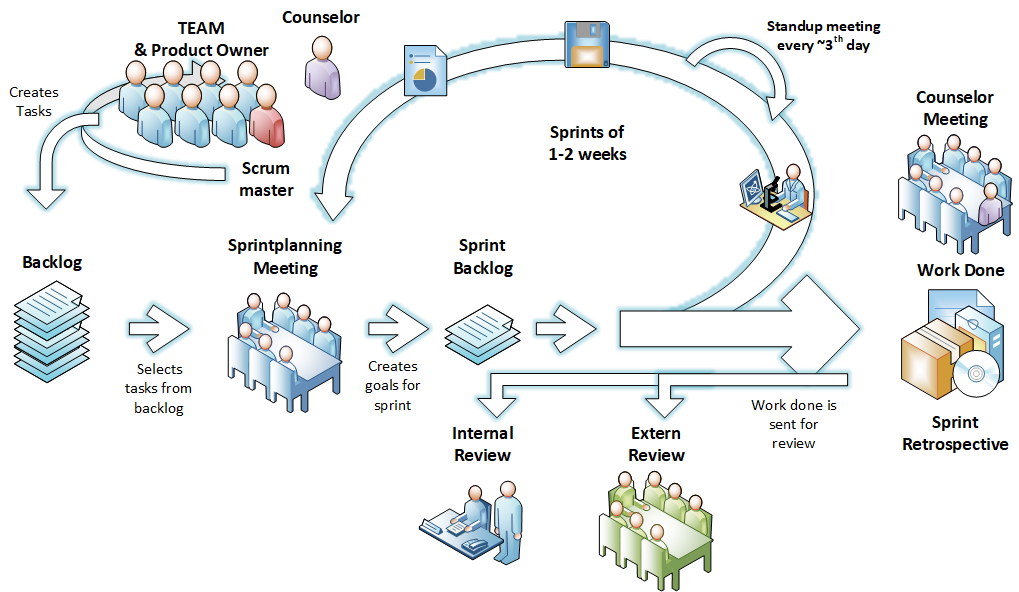
\includegraphics[width=\textwidth]{ProcesDokument/graphics/Scrum_usage.png}
    \caption{Anvendelse af Scrum i projektgruppe 5}
    \label{fig:scrum_usage}
\end{figure}
Af figur \ref{fig:scrum_usage} ses det, hvordan gruppen er deres egne Product Owners, hvordan de laver tasks til backloggen og står for sprint planlægningsmødet. Det ses også, at Sprints har en varighed af 1-2 uger, samt at der er Standup meeting ca. hver 3. dag. Her ses også at noget af det arbejde, der bliver færdiggjort bliver sendt til ekstern review af den anden gruppe eller reviewes internt i gruppen af en review partner. 

Igennem hele projektforløbet har der været eksperimenteret med forskellige metoder for at fremme effektiviseringen og arbejdsindsatsen for projektgruppen. Scrum havde allerede blevet integreret i udviklingsforløbet i et tidligere semester, det var mere specifikke procesfremmende metoder, som blev vurderet:
\begin{itemize}
    \item Hvordan sikre man kvalitet af internt arbejde
    \item Hvordan overholder man de agile principper og værdier
    \item Hvornår er der nok dokumentation til at gå videre til et nyt stadie
    \item Hvordan fremmer man kommunikationen, så man ikke får misforståelser 
\end{itemize}
Dette er nogle af de spørgsmål projektgruppen løbende har eksperimenteret med. Slutproduktet kan som sagt ses i figur \ref{fig:scrum_usage}. De mest essentielle elementer har været de interne reviews, hvor begge parter har samme ansvar for kvaliteten af opgaven (dog kun de større opgaver). Et andet har været at få medlemmer til at udnytte de redskaber, som har været til rådighed(Zenhub, Overleaf, GitHub) - dette vil dog altid tage tid, hvis man ikke har stiftet bekendtskab med det før. Projektgruppen er dog alle enige om, at den iterative tilgang faciliteret af Scrum, er med til at effektivisere arbejdsprocessen, samt sikre et fleksibelt arbejdsmiljø. 

\subsection{Udviklingsværktøjer fra 2., 3. og 4. semester}
I dette afsnit beskrives de udviklingsværktøjer, der blev genanvendt fra 2. og 3. semester. Det drejer sig mere specifikt om ASE-udviklingsmodellen, V-modellen og SysML.
\subsubsection{ASE-Modellen}
ASE modellen er en model introduceret på 2. semester, der kan anvendes til at udvikle et system bestående af hardware og software på en struktureret måde. ASE-modellen ses i figur \ref{fig:ASE}
\begin{figure}[H]
    \centering
    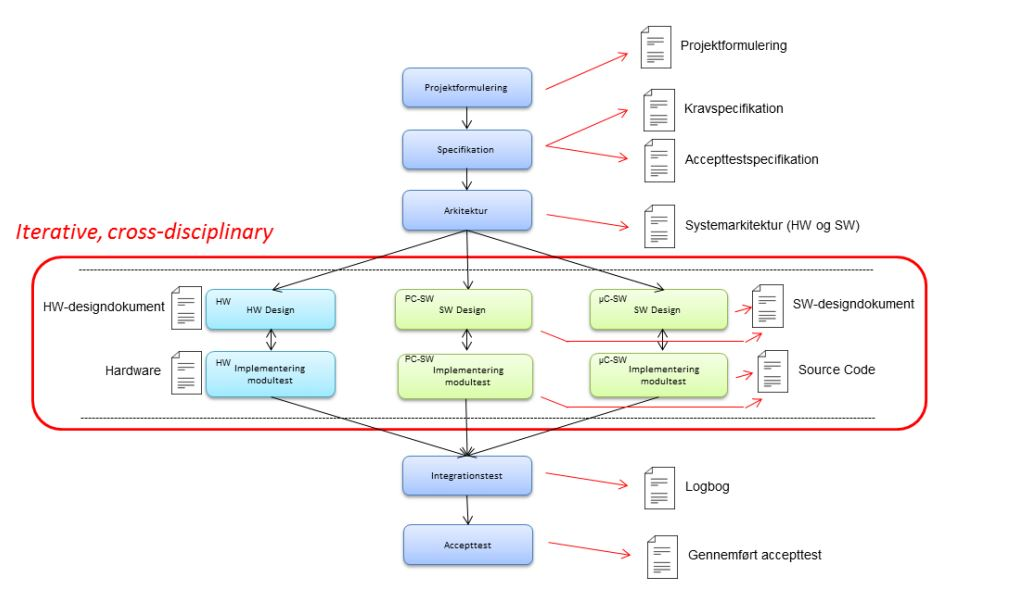
\includegraphics[width=\textwidth]{ProcesDokument/graphics/ASE-Modellen.jpg}
    \caption{ASE-udviklingsmodellen}
    \label{fig:ASE}
\end{figure}
I dette projekt anvendes ASE-Modellen til at danne udviklingen af produktets overordnede struktur. Modellen er ideelt, når man har et godt kendskab til produktets domæne, således det er muligt at gennemgå alle stadierne: Specifikation, Arkitektur, Design mv. Til forskel for modellens angivelse af iterativ disciplin ved blot design- og implementeringsfasen, anvendes en iterativ tilgang ved hele udarbejdelse (Alle stadier) - som nævnt tidligere er det godtroende at antage, at det er muligt at fastsætte krav eller arkitekturen, før man har undersøgt og testet produktet og dets domæne. Processeren beskrevet i ASE-modellen anvendes i flere iterationer, hvor hver iteration ikke nødvendigvis er bundet til en proces; fx kan der godt arbejdes på kravspecifikationen og arkitekturen i samme sprint. 

\subsubsection{SysML}
Til udarbejdelse af de forskellige ASE-processer blev der anvendt SysML, som er et analyse- og designredskab. Her anvendtes en modificeret udgave, der passer til de diagrammer, der har optrådt i 2. semester kurset \textit{Indledende System Engineering}. Den modificerede anvendelse af SysML kan ses i figur \ref{fig:Sysml_usage}.
\begin{figure}[H]
    \centering
    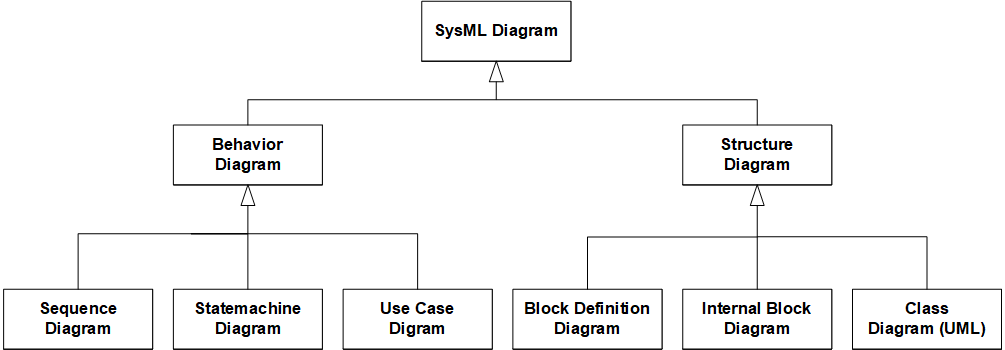
\includegraphics[width=\textwidth]{ProcesDokument/graphics/Sysml_usage.png}
    \caption{Anvendelse af SysML}
    \label{fig:Sysml_usage}
\end{figure}
Af figur \ref{fig:Sysml_usage} ses det, at Sekvens-, Statemachine- og Use Case-diagrammer bruges til at beskrive opførelsen af systemet, hvor Block Definition Diagram og Internal Block Diagram bruges til at beskrive strukturen af systemet. Class diagram fra UML er også inkluderet under struktur, da den beskriver strukturen af software samt relationen mellem de forskellige klasser. 

\section{Projektledelse}
Scrum Masteren har stået for ledelsen i gruppen for de pågældende sprints. Det har været hans ansvar at vide og være i stand til at anvende ledelsesformer, som overholder de agile værdier og principper, der blev nævnt tidligere i dokumentet. Traditionelt set dedikerer Scrum Masteren en stor mængde tid på at sikre, at arbejdsprocessen er optimal og er uddannet til at facilitere dette. Det har dog været tilfældet i dette projekt, at Scrum Masteren har haft lige så meget ansvar for produktetsudførelse som andre medlemmer i projektet. Med det sagt er der dog taget flere overvejelser og aktioner i forhold til arbejdsprocesser i gruppen, ledelse og motivation. 
\begin{displayquote}
"A good process will not save a project from failure if the team doesn’t
have strong players." \\
"A team of average programmers who communicate well are more
likely to succeed than is a group of superstars who fail to interact as
a team."\\ - Martin Fowler
\end{displayquote}
Et projekts største værdi er dets team medlemmer. De er ikke en udskiftelig, og man skal ikke anse deres værdi ud fra deres rolle (Manager, tester, programmør). Fra starten af projektet blev hvert medlem antaget at være professionel, hårdtarbejdende og driftssikker. Det betød, at sprintenes opgaver blev lavet og uddelegeret ud fra denne antagelse. Martin Fowlers artikel 'The New Methology' nævner at det skaber stor motivation at anse hvert medlem som ligeværdige og eksperter indenfor deres specifikke område (Da vi dog alle studerer samme linje, antages at alle medlemmer har samme basisviden fra studiet). Dette skulle angiveligt også skabe en fælles ansvarsfølelse for produktet og dets tekniske aspekter. Scott Ambler beskriver to forskellige slags team i form af software arkitekter: Det kaotiske team og det 
selvorganiserende (se figur \ref{fig:selfChaos}). 
\begin{figure}[H]
    \centering
    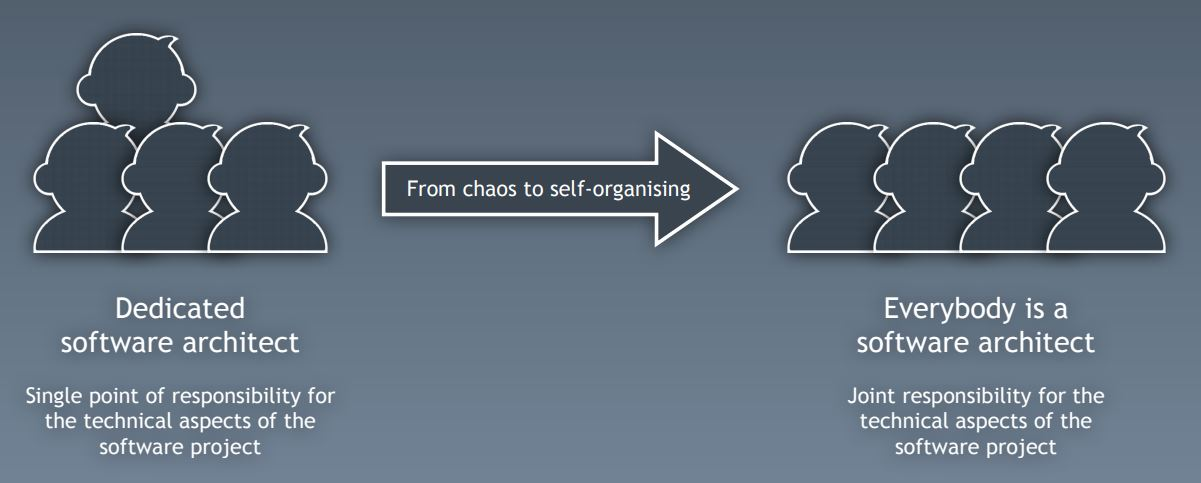
\includegraphics[width=\textwidth]{ProcesDokument/graphics/procesChaos.jpg}
    \caption{From Chaos To Self-organising}
    \label{fig:selfChaos}
\end{figure}
Det ideelle scenario er, når alle medlemmer tager fælles ansvar for produktet og ikke ser deres arbejdsopgaver isoleret fra helheden - man skal løse opgaven med tanken om at tilføje noget produktivt til hele produktet, ikke blot at løse den for at løse den og vise man har lavet noget. \\\\
Den første antagelse om at alle medlemmer har samme karakteregenskaber holdt desværre ikke stik. Der var en stor variation mellem medlemmers præstation, hvor enkelte ikke udtrykte den samme form for ansvarsobligation, som aftalt ved starten af projektet. For at motivere selvsagte medlemmer blev forskellige metoder anvendt. \\\\
\textbf{Tillid og anerkendelse:}\\
Hvis opgaver ikke blev lavet i et sprint, blev medlemmet konfronteret og spurgt grunden til manglende arbejdsindsats. Herefter blev der ofte givet en mulighed for at færdiggøre arbejdsopgaver i det næste sprint, hvor færre opgaver blev givet til det nye sprint for medlemmet.  Dette skulle selvfølgelig ikke ske ofte, da det kan give anledning som motivation til at netop ikke færdiggøre ens opgaver for at have en lettere arbejdsbyrde. \\
Hvis medlemmet færdiggjorde arbejdsopgaven tilfredsstillende, blev der givet stor anerkendelse for arbejdet. Fremover vil der ikke blive stillet spørgsmål til medlemmets arbejdsindsats medmindre, der gives anledning til det. \\\\
\textbf{Konsekvens:}\\
Hvis et medlem gentagne gange ikke færdiggør eller påbegynder deres opgaver, konfronteres medlemmet. Dette er et fælles akademisk projekt, og alle bedømmes ud fra det færdige projekt - ligeledes alle andre projekter, vil et medlems udfald påvirke alle andres. Medlemmet skal selvfølgelig ikke belønnes af andres arbejde til eksamen, hvis personen ikke har bidraget. Hvis denne situation opstår, opfordres medlemmer stærkt at tage sig sammen, ellers inddrages medlemmet til samtale med vejleder. Hvis opførslen fortsættes vil gruppen være nødsaget til at fjerne medlemmet fra projektet \\\\
Motivations- og ledelsemetoderne er dog desværre begrænset ud fra Scrum Masterens egen viden og det litteratur udleveret i undervisning (Martin Fowler \& Scott Ambler). Det ville angiveligt have været optimalt, hvis der havde været brugt flere ressourcer på proces og ledelse, idet det fremmer kommunikationen og det generelle projekt. Vi var dog alle enige om, at vi ville prioritere selve produktet. 

\section{Arbejdsfordeling}
En er de vigtigske elementer af Scrum, er fleksibiliteten ved at påtage opgaver - såkaldte task ofte bliver lavet ud fra 'mindre' funktionalitet, da det skal kunne udføres i et sprint med en varighed på 1-2 uger. Projektets tekniske aspekter indgår ofte under det undervisningsmateriale, som er gennemgået, hvert medlem burde således have ekspertisen til at udføre alle opgaver - der vil dog komme et tidspunkt, hvor enkelte medlemmer har brugt en del ressourcer på at undersøge nye teknologier eller løsninger, hvor det ikke giver mening at tilføje medlemmer, som ikke har denne viden. Der tildeles en reviewpartner til hvert opgave, som nødvendigvis ikke har samme ekspertisen, på den måde kan alle medlemmer blive inddraget i de forskellige elementer. Nedenfor ses en tabel, som angiver den overordnet arbejdsfordeling. \\\\
Generelt set har alle substantielle taks være uddelegeret til minimum to medlemmer, således at der næsten altid er en til rådighed, samt to forskellige perspektiver på et problem 
\section{Ansvarsområder}
\begin{longtable}{|L{0.2\textwidth}|L{0.082\textwidth}|L{0.08\textwidth}|L{0.08\textwidth}|L{0.08\textwidth}|L{0.08\textwidth}|L{0.08\textwidth}|L{0.08\textwidth}|L{0.08\textwidth}|}
        \hline
        \textbf{Ansvarsområde}  &\textbf{HBA}   &\textbf{TM}    &\textbf{MGJ}   &\textbf{MH}    &\textbf{EB}    & \textbf{AE}  & \textbf{MG}   &\textbf{EM}      \\ \hline
        Resume / abstract       &               &               &               &               &               &               &               &                \\ \hline
        Forord                  &               &               &               &               &               &               &               &                \\ \hline
        Indledning              &               &               &               &               &               &               &               &                \\ \hline
        Projektformulering      &               &               &               &               &               &               &               &                \\ \hline
        Funktionelle krav       &               &               &               &               &               &               &               &                \\ \hline
        Ikke-funktionelle krav  &               &               &               &               &               &               &               &                \\ \hline
        Afgrænsning             &               &               &               &               &               &               &               &                \\ \hline
        Metode og Proces        &               &               &               &               &               &               &               &                \\ \hline
        Analyse                 &               &               &               &               &               &               &               &                \\ \hline   
        System Arkitektur       &               &               &               &               &               &               &               &                \\ \hline
        System Sekvensdiag.     &               &               &               &               &               &               &               &                \\ \hline
        Grænseflader            &               &               &               &               &               &               &               &                \\ \hline
        Software Arkitektur     &               &               &               &               &               &               &               &                \\ \hline
        GUI                     &               &               &               &               &               &               &               &                \\ \hline
        Database                &               &               &               &               &               &               &               &                \\ \hline
        Integrationstest        &               &               &               &               &               &               &               &                \\ \hline
        Accepttest              &               &               &               &               &               &               &               &                \\ \hline
        Konklusion              &               &               &               &               &               &               &               &                \\ \hline 
        Fremtidigt arbejde      &               &               &               &               &               &               &               &                \\ \hline
\caption{Ansvarsområder for medlemmer af PRJ3 Gruppe 7, hvor \textbf{P} indikerer at medlemmet har været primæraktør og \textbf{S} indikerer at medlemmet har været sekundæraktør}
\end{longtable}
Her er det vigtigt at pointere, at dette er kun et overordnet billede af arbejdsfordelingen. Der er også lagt mange arbejdstimer i andre forbindelser af projektet. 

\section{Planlægning}
I starten af projektet blev det vurderet, hvorvidt det var nødvendigt at lave en tidsplan for projektets forskellige stadier - fx første udkast af kravspecifikationen skal være færdig i sprint 2. De fleste projektmedlemmer havde dårlig erfaring med en tidsplan. Enten blev den aldrig brugt, eller så var den utrolig misvisende - det er svært at angive en statisk tidsplan for et softwareprojekt. Det blev derfor bestemt, at det var Scrum Masterens opgave at sørge for at alle deadlines blev nået (Både dem angivet af Aarhus Universitet og interne i gruppen). De tidligere sprint blev ofte givet et tema, som var associeret med et af ASE-processerne. Alle parter var dog enige om, at det ville være ideelt at have første udkast af rapport og dokumentation færdig en uge før afleveringsdeadline (d. 28. maj 2019). I det næste afsnit beskrives, hvordan den iterative planlægning blev planlagt i forhold til selvsagte deadlines. 

\subsection{Iterativ Planlægning}
Det var et krav at anvende en iterativ udviklingsproces. Sprintene blev brugt som driftscykluser, hvor man gerne skal komme tættere på det ønskede produkt efter hvert itereation. Til forskel fra det forrige semester, hvor der var en del flere reviews og andre deadlines, så har der kun været et officielt review i dette semesterprojekt, hvilke lå tidligt i arbejdsprocessen. Dette betød, at fremover ville planlægningen være inspireret af de agile principper i forhold til at kravspecifikation, og arkitekturen kun skal dokumenteres, således alle var indforstået. Planlægningen blev mere fælles orienteret, da alle var en del udviklingsfasen - det var Scrum Masterens rolle at sørge for, at projektet langsom realiseres, således det er klar til aflevering d. 28. maj (Produkt og dokumentation) 

\section{Møder}
I dette afsnit beskrives overordnet set de møder, der har været i forbindelse med projektet. Møderne vil ikke beskrives hver især, men der henvises til Vejledermøde- og Gruppemøde-dokument. Der var et møde hver mandag og onsdag kl. 12.15, og Scrum Masteren havde minimum lavet en dagsorden 24 timer før, hvor de andre projektmedlemmer havde mulighed for at tilføje punkter, som skulle behandles til mødet.  I de følgende afsnit vil de forskellige typer af møder beskrives overordnet 

\subsection{Vejledermøder}
Hvert onsdag kl. 12.15 var der afsat en time til sparring med vejlederen. Det var Scrum Masterens ansvar at få indsamlet talepunkter fra gruppemedlemmerne og sende en dagsorden til vejlederne dagen forinden. Møderne blev generelt brugt til at opdatere vejlederen om projektets status, men ved enkelte lejligheder, havde gruppen sendt dokumentation til review. Hvis gruppen havde behov for feedback fra vejlederen i forhold til deres dokumentation, skulle det sendes minimum 4 arbejdsdage før mødet. Faglige og tekniske spørgsmål blev henvist til undervisere i de pågældende tekniske discipliner. Til hvert møde var der en referent - denne rolle gik på tur mellem gruppens medlemmer. 

\subsection{Gruppemøder}
Dette var de interne møder i gruppen, hvor der blev arbejdet på projektet. I starten af projektet blev gruppemøderne brugt meget til at gennemgå forskellige dokumenter eller diagrammer i fællesskab, for at skabe en fælles forståelse for systemet og samtidig sikre, at kvaliteten på dokumenterne var høj fra en start af. Senere hen i processen udviklede disse gruppemøder sig mere til at arbejde på implementeringsaspekter i fællesskab. Herved var det sikret, at man brugt arbejdstid på projektet, men også at hvis der skulle opstå problemer, så havde man mulighed for at få hjælp af et andet gruppemedlem. Den sidste mandag i hvert sprint blev brugt til at reviewe andres arbejde, på den måde havde vi en form for kvalitetssikring og feedbacksystem allerede for begyndelsen af projektet. I starten blev reviewet dog ikke realiseret, da der ikke blev uddelegeret en specifik review person til hver opgave - det var således medlemmetz, som havde lavet opgaven, ansvar at finde en reviewpartner. I et af de senere sprint blev der tildelt en reviewpartner til næste alle opgaver, som også havde ansvaret for opgaven - dvs. hvis opgaven ikke blev lavet tilfredsstillende, eller overhovedet lavet, så stod de begge til ansvar. 

\subsection{Review}
Der var et planlagt reivewmøde for hele semesterprojektet. Gruppen blev tildelt gruppe 6, som skulle give feedback på vores kravspecifikation. Mødets forløb var at først lavede den ene gruppe et review, mens den anden gruppe modtog konstruktiv kritik uden at stille for mange spørgsmål og derefter blev rollerne byttet. Dette møde var en øjenåbner for os, da vi havde alt for store ambitioner for projektet. Efter mødet afgrænsede vi projektets omfang substantielt. 

\section{Konflikthåndtering}
...

\printbibliography
\end{document}